\section{Zielsetzung}
\label{sec:Zielsetzung}
In diesem Versuch soll die Wellenlänge eines Lasers mit Hilfe des Michelson-Interferometers bestimmt werden.
Mit selbigem Versuchsaufbau ist weiter der Brechungsindex von Luft zu bestimmen.

\section{Theorie}
\label{sec:Theorie}

Um den Aufbau und die Funktionsweise des Michelson-Interferometeres zu erläutern, 
muss zuerst der grundlegende Begriff der Interferenz näher erklärt werden. Licht
ist eine elektromagnetische Welle, deren Ausbreitung sich mit den Maxwell-Gleichungen
beschreiben lässt. Im Allgemeinen lässt sich die orts- und zeitabhängige ($x,t$) elektrische Feldstärke einer solchen Welle mit

\begin{align}
\vec{E}(x,t) = \vec{E_\text{0}} \cos(kx - \omega t - \delta)
\end{align}

darstellen, wobei $k = \frac{2\pi}{\lambda}$ die Wellenzahl mit $\lambda$ als Wellenlänge, $\omega$ die Kreisfrequenz
und $\delta$ einen beliebigen Phasenwinkel repräsentieren. Für solche Gleichungen gilt das Superpositionsprinzip,
sodass sich zwei (oder mehr) an einem Ort $P$ ankommende Wellen überlagern und die Feldstärke addiert werden kann.
Da sich aufgrund der hohen Frequenz der genutzten Lichtquelle allerdings besser die Lichtintensität 

\begin{align*}
I = \mathrm{const} |\vec{E}|^{2}
\end{align*}

beobachten lässt, ergibt sich für die Addition zweier Wellen

\begin{align}
I_\text{ges} = 2 \mathrm{const} \vec{E_\text{0}}^{2} (1 + \cos(\delta_\text{2} - \delta_\text{1})).
\end{align}

\noindent Hierbei wird deutlich, dass der zweite Teil der Summe, welcher Interferenzterm genannt wird, abhängig von der
Phasenbeziehung $(\delta_\text{2} - \delta_\text{1})$ ist und somit Werte von $-2 \mathrm{const} \vec{E_\text{0}}^{2}$ bis 
$2 \mathrm{const} \vec{E_\text{0}}^{2}$ annehmen kann. Insbesondere verschwindet er bei einer Phasenverschiebung von einem
ungeraden Vielfachen von $\pi$. Aufgrund der statistischen Natur der Entstehung von Licht lässt sich somit aus Licht
zweier verschiedener Lichtquellen im Allgemeinen keine Interferenz beobachten. Es wird von inkohärentem Licht gesprochen.
Kohärentes Licht, welches beispielsweise mit einem Laser erzeugt werden kann, besitzt gemäß Gleichung (1) ein festes $k$, 
$\omega$ und $\delta$ für alle emittierten Wellenzüge. Wird kein Laser, sondern eine konventionelle Lichtquelle verwendet,
sind eine Bedingungen für eine Kohärenz gegeben. Wichtig ist die Kohärenzlänge 
\begin{align}
l = N \lambda,
\end{align}
welche die maximale Länge entlang eines interferenzfähigen Wellenzuges beschreibt. Wird zudem die Ausbreitungsgeschwindigkeit 
zweier Teilbündel betrachtet und mithilfe einer Fouriertransformation die Breite der Beugungsmaxima bestimmt,
folgt für diese
\begin{equation*}
  \Deltaa \lambda = \frac{\lambda_0^2}{c \tau}.
\end{equation*}
Die Kohärenzzeit ist
\begin{equation*}
  \tau = \frac{l}{c},
\end{equation*}
womit sich
\begin{equation}
  \Deltaa \lambda = \frac{\lambda_0^2}{l}
\end{equation}
ergibt.
Für eine reale, ausgedehnte Lichtquelle sind entweder die Ausdehnung oder der Öffnungswinkel einzuschränken, um Interferenzeffekte beobachten zu können,
da diese eine eigene Phasenverschiebung verursachen, welche die eigentlich zu beobachtbare Interferenz beeinträchtigt.
Abbildung \ref{fig:ausgedehnt} ist die geometrische Beziehung
\begin{equation}
\Deltaa \phi = \frac{2\pii}{\lambda}a \sin(\gamma)
\end{equation}
zu entnehmen.
\begin{figure}
  \centering
  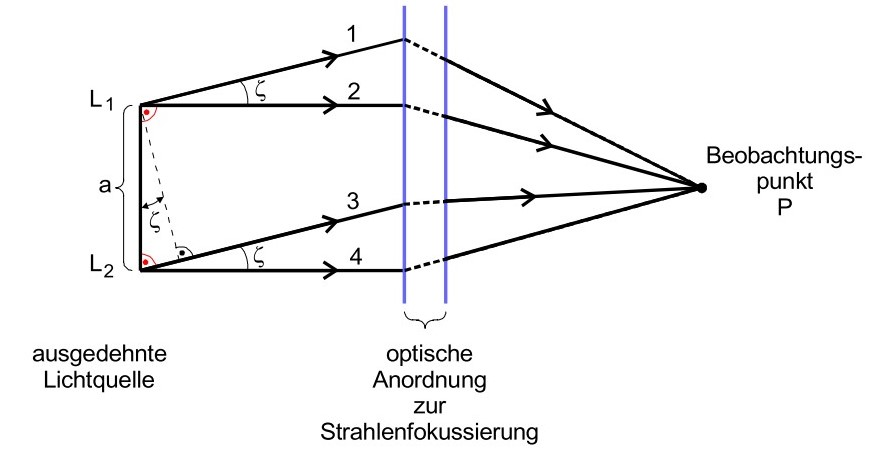
\includegraphics{graphics/ausgedehnt.jpg}
  \caption{Strahlengang einer ausgedehnten Lichtquelle \cite{Anleitung}.}
  \label{fig:ausgedehnt}
\end{figure}
Als Kohärenzbedingung für ausgedehnte Lichtquellen folgt aus der Bedingung $\Deltaa \phi \ll \pii$ die Ungleichung
\begin{equation}
  a \sin(\gamma) \ll \frac{\lambda}{2}.
\end{equation}
So wird der Öffnungswinkel leicht durch einen großen Abstand zur Lichtquelle realisiert.
